% Created 2017-07-12 Wed 11:53
\documentclass[presentation]{beamer}
\usepackage[utf8x]{inputenc}
\usepackage[T1]{fontenc}
\usepackage{fixltx2e}
\usepackage{graphicx}
\usepackage{longtable}
\usepackage{float}
\usepackage{wrapfig}
\usepackage{rotating}
\usepackage[normalem]{ulem}
\usepackage{amsmath}
\usepackage{textcomp}
\usepackage{marvosym}
\usepackage{wasysym}
\usepackage{amssymb}
\usepackage{hyperref}
\tolerance=1000
\usepackage{minted}
\usetheme{metropolis}
\setbeamertemplate{frame footer}{Erwin Rooijakkers}
\metroset{block=fill}
\usetheme{default}
\author{Erwin Rooijakkers}
\date{12-07-2017}
\title{Blockchain, Smart Contracts, ClojureScript, Fleet}
\hypersetup{
  pdfkeywords={},
  pdfsubject={},
  pdfcreator={Emacs 25.1.1 (Org mode 8.2.10)}}
\begin{document}

\maketitle

\section{Blockchain}
\label{sec-1}

\begin{frame}[label=sec-1-1]{Initial Coin Offering (ICO) announcement}
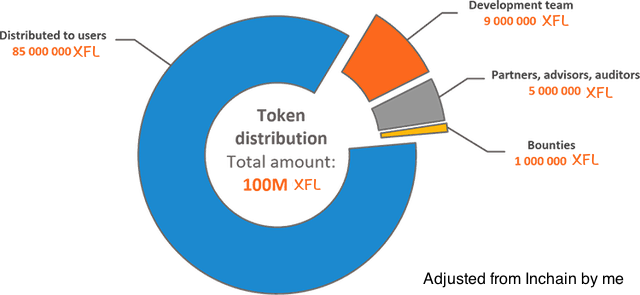
\includegraphics[width=.9\linewidth]{../images/ico.png}
\end{frame}
\begin{frame}[label=sec-1-2]{Blockchain?}
\begin{quotation}
"A \alert{shared}, programmable, cryptographically secure and therefore trusted ledger
\alert{which no single user controls} and \alert{which can be inspected by everyone}."

-- Klaus Schwab (Chairman World Economic Forum)
\end{quotation}
\end{frame}

\begin{frame}[label=sec-1-3]{Four pillars}
\begin{itemize}
\item Cryptographic Tokens and Addresses
\item P2P Networking
\item Consensus Formation Algorithm
\item Virtual Machine
\end{itemize}
\end{frame}

\begin{frame}[label=sec-1-4]{This.}
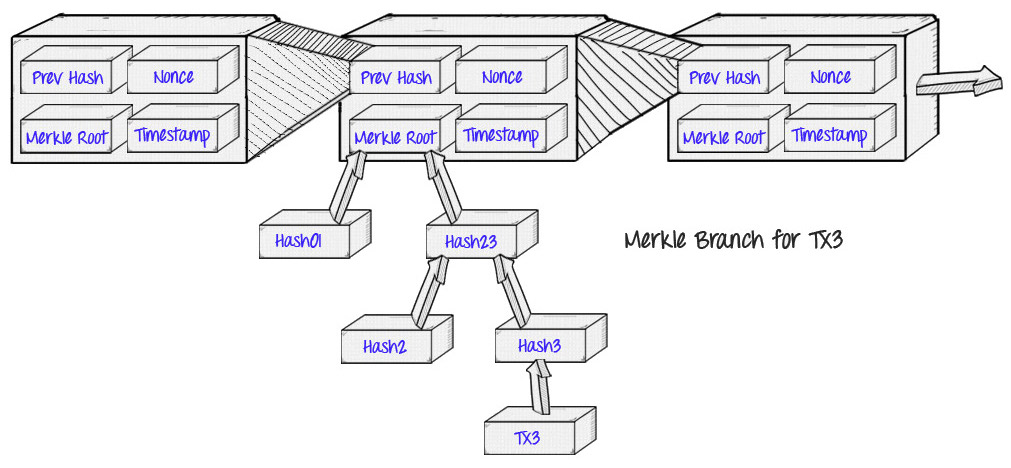
\includegraphics[width=.9\linewidth]{../images/merkle.jpg}

Source: \url{https://blog.ethereum.org/2015/11/15/merkling-in-ethereum/}
\end{frame}

\begin{frame}[label=sec-1-5]{Consensus}
\begin{itemize}
\item Proof of Work (\alert{PoW})
\end{itemize}
\begin{itemize}
\item Proof of Stake (\alert{PoS})
\end{itemize}
\end{frame}

\section{Smart Contracts}
\label{sec-2}

\begin{frame}[label=sec-2-1]{Business logic in decentralized network}

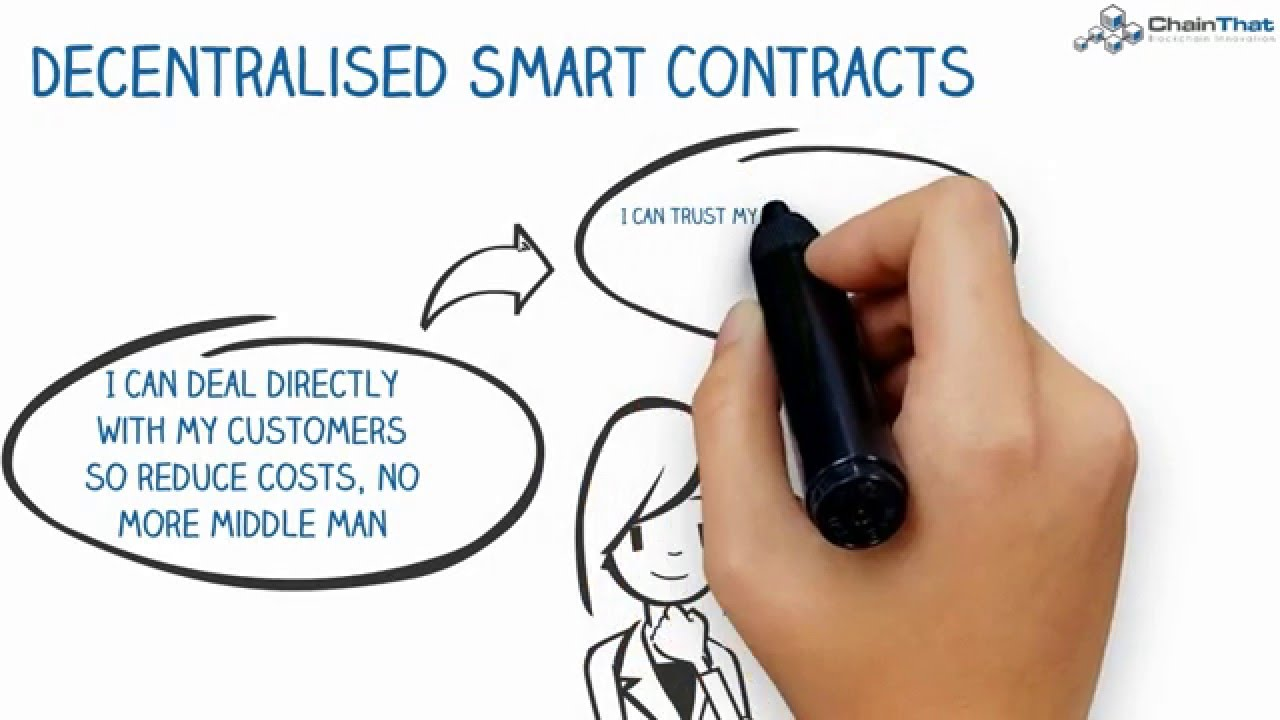
\includegraphics[width=.9\linewidth]{../images/smartcontract.jpg}

Source: ChainThat YouTube video
\end{frame}

\begin{frame}[label=sec-2-2]{Model}
\begin{itemize}
\item Stateless webservices
\item Contract-oriented programming
\item Gas fees
\end{itemize}
\end{frame}

\begin{frame}[label=sec-2-3]{Stateless webservices}
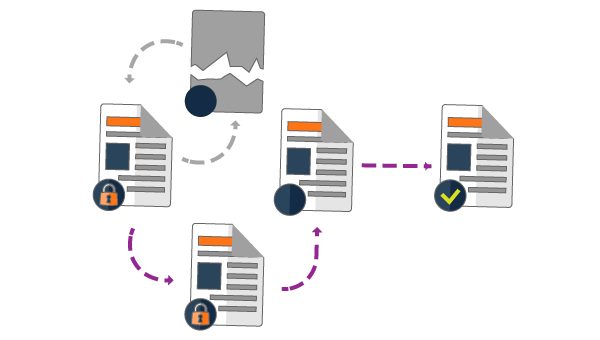
\includegraphics[width=.9\linewidth]{../images/smartcontracteth.png}

Source: ETH news
\end{frame}

\begin{frame}[label=sec-2-4]{Stateless web services}
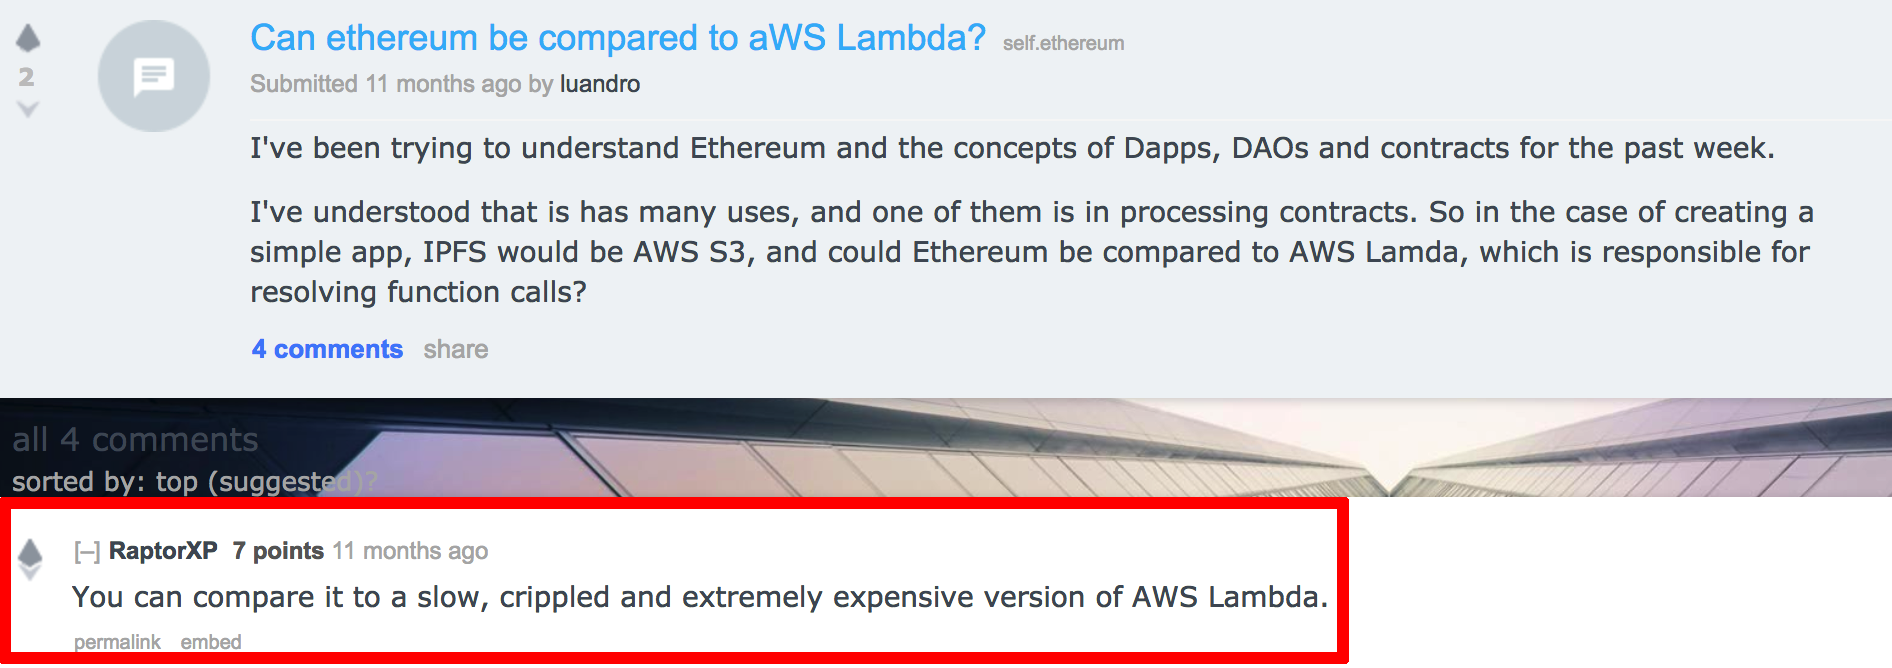
\includegraphics[width=.9\linewidth]{../images/awslambda.png}
\end{frame}

\begin{frame}[fragile,label=sec-2-5]{Contract-oriented programming}
 \begin{minted}[bgcolor=white,frame=lines]{javascript}
contract HelloSayerFactory {

  function create() returns (address) {
    return address(new HelloSayer());
  }

  function delete(address addr){
    HelloSayer(addr).remove();
  }

}
\end{minted}
\end{frame}

\begin{frame}[label=sec-2-6]{Tools}
\begin{itemize}
\item geth: (Go Ethereum) \alert{cli} for running full Ethereum node, exposes RPC
\item web3.js: Ethereum compatible \alert{JavaScript API} which implements the Generic \alert{JSON RPC spec}
\item solc: JavaScript bindings for Solidity compiler (creates \alert{ABI} and \alert{BIN})
\end{itemize}
\end{frame}

\begin{frame}[label=sec-2-7]{MetaMask (also: Mist; Parity)}

\includegraphics[width=.9\linewidth]{../images/metamask.png}
\end{frame}

\section{Fleet}
\label{sec-3}
\begin{frame}[label=sec-3-1]{Why ClojureScript + blockchain}
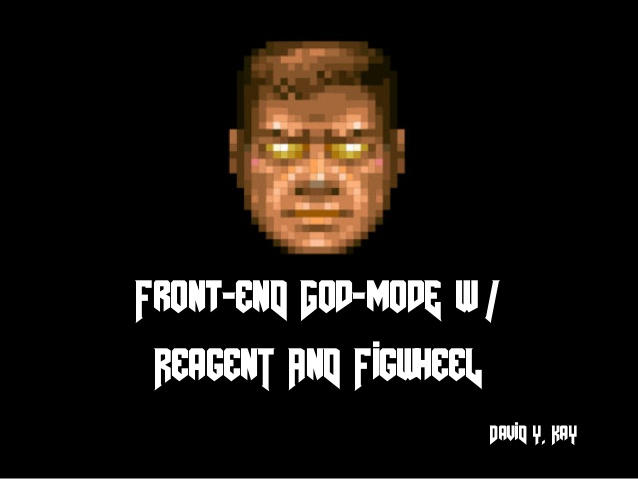
\includegraphics[width=.9\linewidth]{../images/godmode.jpg}
\end{frame}

\begin{frame}[label=sec-3-2]{Code inspiration and big help}
\begin{itemize}
\item \url{https://medium.com/@matus.lestan}
\item \url{https://github.com/district0x/ethlance}
\item \url{https://ethlance.com/\#/job/128}
\end{itemize}

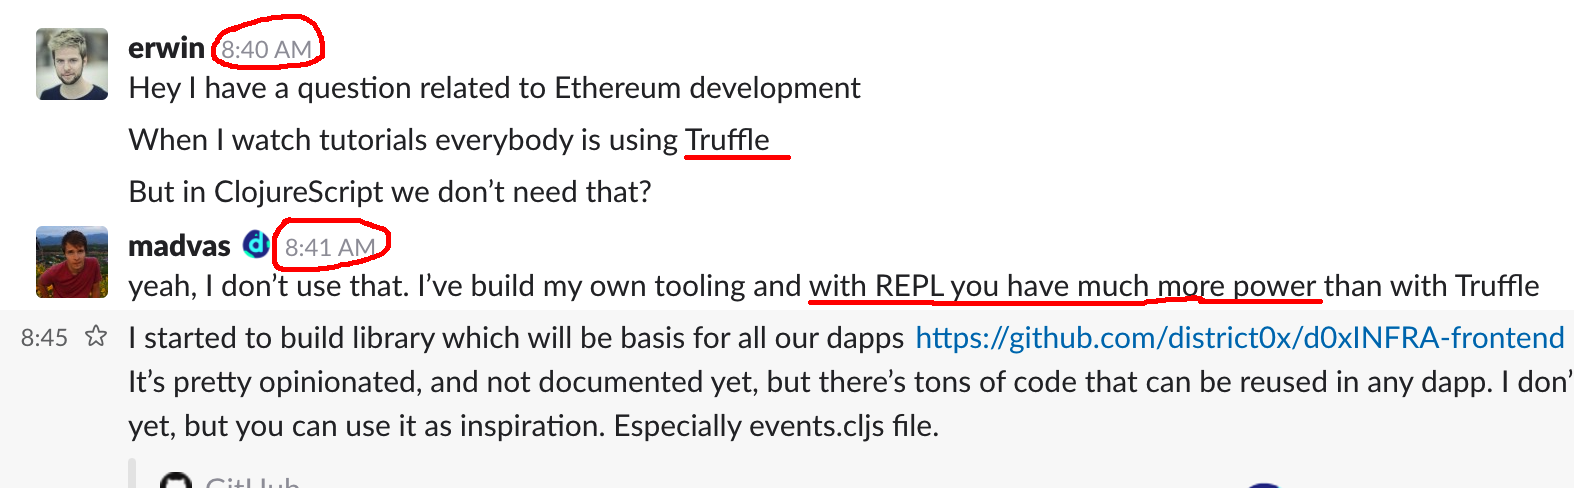
\includegraphics[width=.9\linewidth]{../images/madvas.png}
\end{frame}
\begin{frame}[label=sec-3-3]{Idea}
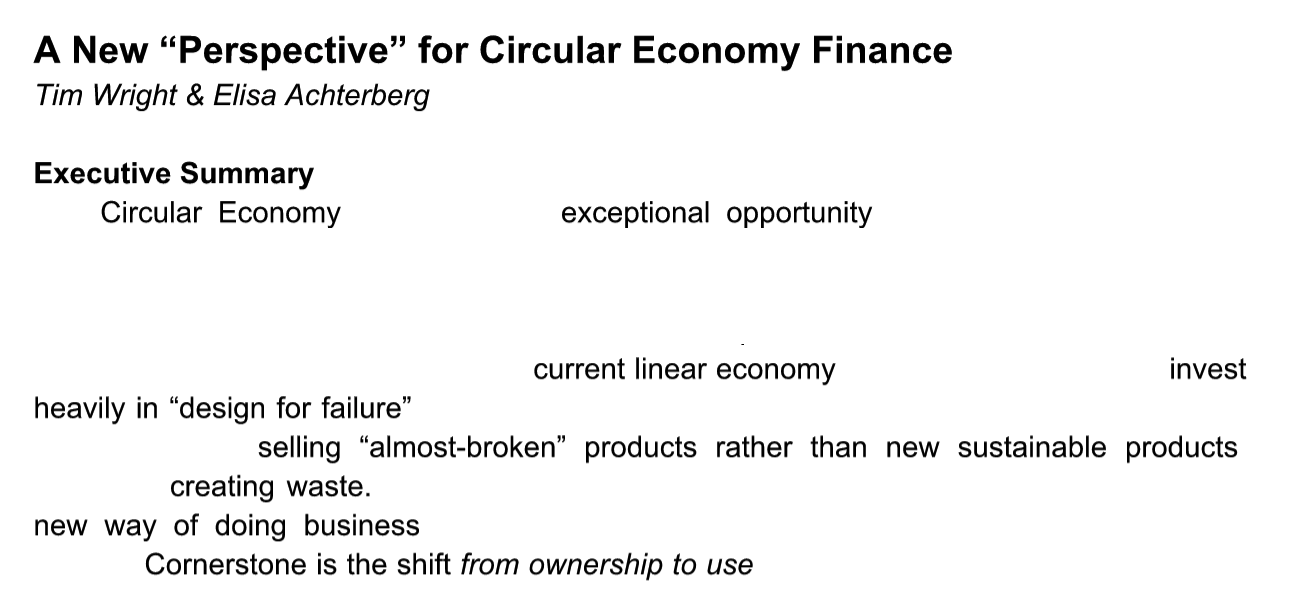
\includegraphics[width=.9\linewidth]{../images/circular.png}
\end{frame}

\begin{frame}[label=sec-3-4]{Linear economy designs for failure}
\includegraphics[width=.9\linewidth]{../images/politico.jpg}

Source: Politico Europe
\end{frame}

\begin{frame}[label=sec-3-5]{Smart assets}
\begin{itemize}
\item When they are used, \alert{smart assets} (a \alert{\uline{fleet}} of assets) pay parties
involved in value chain (involved with design, commodities, creation,
maintenance, et cetera)
\end{itemize}
\end{frame}

\begin{frame}[label=sec-3-6]{Shift from ownership to use}
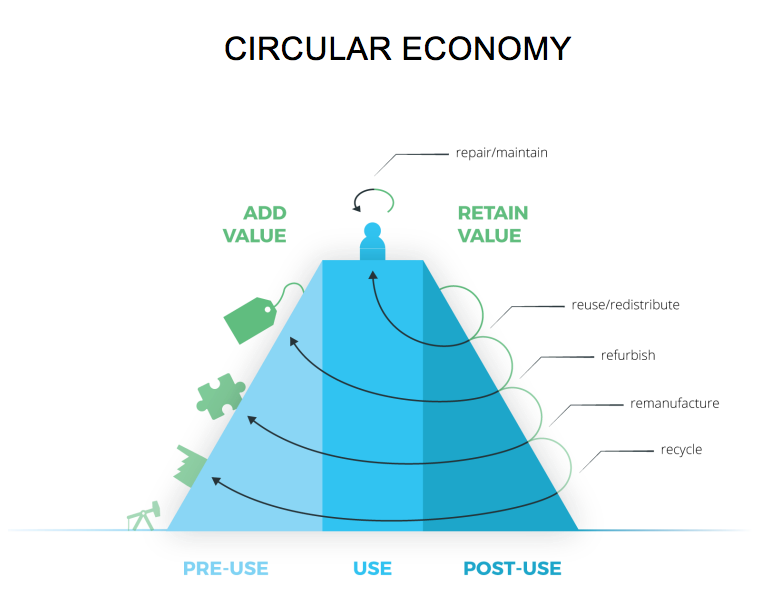
\includegraphics[width=.9\linewidth]{../images/circulareconomy.png}

Source: Circle Economy
\end{frame}

\begin{frame}[label=sec-3-7]{Contract design}
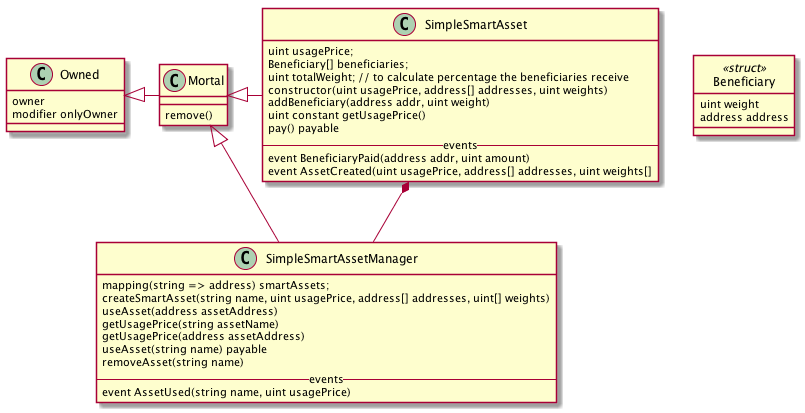
\includegraphics[width=.9\linewidth]{../images/fleet.png}
\end{frame}

\begin{frame}[label=sec-3-8]{App design}
\begin{itemize}
\item Reagent atom for \alert{application state}:
\begin{itemize}
\item Frontend state: (beneficiaries)
\item Blockchain state: Contract instance, abi and bin
\item Address of user
\item \alert{queries.cljs} to interact with ratom
\item \alert{views.cljs} reacts to its changes $v=f(S)$, or something
\end{itemize}

\item \alert{blockchain.cljs} \emph{deploys} or \emph{retrieves} contracts
\begin{itemize}
\item Depending on network of web3 object (Ropsten or local)
\end{itemize}
\item \alert{smart\textunderscore{}asset\textunderscore{}manager.cljs} calls methods on instances
\item Both use the \alert{web3-cljs} web3.js wrapper

\item Setup local blockchain for development with \alert{fleet.el}
\item TODO: \alert{tests}\ldots{}, \alert{IPFS} deployment
\end{itemize}
\end{frame}

\section{Fleet demo}
\label{sec-4}
% Emacs 25.1.1 (Org mode 8.2.10)
\end{document}
